On considère les fonctions $f_k$ définies sur $\R$ par $f_k(x)=x + k\,\e^{-x}$, où $k$ est un réel strictement positif.

\begin{enumerate}
	\item On s’intéresse dans cette question au cas $k = 0,5$, donc à la fonction $f_{0,5}$ définie sur $\R$ par \[f_{0,5}(x)=x + 0,5\,\e^{-x}.\]
	\begin{enumerate}
		\item Montrer que la dérivée de $f_{0,5}$ notée $f'_{0,5}$ vérifie $f'_{0,5}(x) = 1-0,5\,\e^{-x}$.
		\item Montrer que la fonction $f_{0,5}$ admet un minimum en $\ln(0,5)$.
	\end{enumerate}
\end{enumerate}

Soit $k$ un réel strictement positif. On donne le tableau de variations de la fonction $f_k$.

\begin{center}
	\begin{tikzpicture}
		\tkzTabInit[lgt=4]{Valeurs de $x$/1,Variations de $f_k$/2}{$-\infty$,$\ln(k)$,$+\infty$}
		\tkzTabVar{+/$+\infty$,-/$f_k(\ln(k))$,+/$+\infty$}
	\end{tikzpicture}
\end{center}

\begin{enumerate}[resume]
	\item Montrer que pour tout réel positif $k$, $f_k(\ln(k)) = \ln(k) + 1$.
\end{enumerate}

On note $\Courbe[k]$ la courbe représentative de la fonction $f_k$ dans un plan muni d’un repère orthonormé.

On note $A_k$ le point de la courbe $\Courbe[k]$ d’abscisse $\ln(k)$.

\smallskip

On a représenté ci-dessous quelques courbes $\Courbe[k]$ pour différentes valeurs de $k$.

\begin{center}
	\begin{tikzpicture}[xmin=-4,xmax=9,ymin=0,ymax=9]
		\AxesTikz[ElargirOx=0,ElargirOy=0]
		\AxexTikz{-4,-3,...,8}\AxeyTikz{1,...,8}
		\FenetreTikz
		\foreach \k in {0.5,1,1.5,2,2.5,3,3.5,4,4.5,5}{%
			\CourbeTikz[very thick,darkgray,samples=500]{\x+\k*exp(-\x)}{\xmin:\xmax}
			\filldraw[darkgray] ({ln(\k)},{ln(\k)+\k*exp(-ln(\k))}) circle[radius=2pt] ;
		}
		\draw[darkgray] ({ln(0.5)},{ln(0.5)+0.5*exp(-ln(0.5))}) node[above=1pt,inner sep=1pt,font=\footnotesize] {$A_{0,5}$} ;
		\draw[darkgray] ({ln(1)},{ln(1)+1*exp(-ln(1))}) node[right=1pt,inner sep=1pt,font=\footnotesize] {$A_{1}$} ;
		\draw[darkgray] ({ln(1.5)},{ln(1.5)+1.5*exp(-ln(1.5))}) node[above=1pt,inner sep=1pt,font=\footnotesize] {$A_{1,5}$} ;
		\draw[darkgray] ({ln(5)},{ln(5)+5*exp(-ln(5))}) node[above=1pt,inner sep=1pt,font=\footnotesize] {$A_{5}$} ;
	\end{tikzpicture}
\end{center}

\begin{enumerate}[resume]
	\item Indiquer si l’affirmation suivante est vraie ou fausse. Justifier la réponse. Une réponse non justifiée ne rapporte aucun point.
	
	\begin{itemize}
		\item \textbf{Affirmation :} « Pour tout réel $k$ strictement positif, les points $A_{0,5}$, $A_{1}$ et $A_k$ sont alignés. »
	\end{itemize}
\end{enumerate}